\providecommand{\setflag}{\newif \ifwhole \wholefalse}
\setflag %create new if variable name ifwhole(whole)  
\ifwhole\else %if whole flag is set to true do nothing else do codes below

  \documentclass[12pt,a4paper,oneside,hidelinks]{book}

    %\input{extra_package.tex}
    %\input{tweak.tex}
    %\input{commando.tex}
    %\input{font}
  \newcommand\thesisDir{/home/asl/version-control/ws_thesis/thesis_latex}
  \usepackage{import}
  %\usepackage{natbib}
  \usepackage[backend=biber,bibencoding=utf8,style=authoryear]{biblatex}
  \addbibresource{\thesisDir/bibtex/library.bib}
	\usepackage{soul,color}
  \usepackage{pdflscape} %for changing page orientation
  \usepackage[shortlabels]{enumitem}
  \usepackage{amssymb}
  \usepackage{graphicx} %for inserting photo
  \usepackage{subcaption}
  \usepackage{amsmath} % for equations
  \DeclareMathOperator*{\argmax}{argmax} % for underword argmax

  \usepackage{mathtools} % for equations
  \usepackage{physics}


  \usepackage{float}  %deactivate this if hyperref does not work with algo
  \usepackage{hyperref}
  \usepackage{tocbibind}  
  \usepackage[linesnumbered,ruled,vlined]{algorithm2e}
  \usepackage{titlesec} %for deeper subsections and changing chpt sec style
  \setcounter{secnumdepth}{4} %setting subsection 4 section deep
  % numbering equations
  \ifwhole
    \numberwithin{equation}{chapter} %equation number based on chapter
  \else
%    \numberwithin{equation}{section} % equation number based on section
  \fi

  \usepackage{xfrac} % for fraction in the for n/d
  \usepackage{esint} % for easy integral symbols

  %for listing algorithms from algorithm2e
  \newcommand{\listofalgorithmes}{\tocfile{\listalgorithmcfname}{loa}}
  %for footnote
  \renewcommand{\thefootnote}{\fnsymbol{footnote}}

  % for formattgin algorithm2e box [iman] I have to put after listofalgorithmes
  \newcommand\mycommfont[1]{\footnotesize\ttfamily\textcolor{blue}{#1}}
  \SetCommentSty{mycommfont}
  \SetKwInput{KwInput}{Input}                % Set the Input
  \SetKwInput{KwOutput}{Output}              % set the Output

  % This command is usefule when importing subdirectory items
  %margin
\usepackage{setspace}
\usepackage[
  a4paper,
  left=3.8cm,
  right=2.5cm,
  top=2.5cm,
  bottom=3cm,
  footskip=1.7cm
]
{geometry}

%IIUM font size
%syntax {\TITLEfontsize IIUM idiotize thesis formatting }
\newcommand\TITLEfontsize{\fontsize{17pt}{20.4pt}\selectfont}
\newcommand\CHAPTERfontsize{\fontsize{14pt}{16pt}\selectfont}
%For line over line for signature
\usepackage{calc}
\newcommand{\sigline}[1]{\makebox[\widthof{#1~}]{.\dotfill}\\#1}
%another over line signature command
%syantax \sign{The signant name} 
%syntax \Date but use it within minipage
%\begin{minipage}[t]{0.4\linewidth}
%    \raggedright
%    \sign{Supervisor}
%    \par
%    Mr.\,L. L. Silva\par
%    Department of Computing and Information Systems, \par
%    Faculty of Applied Sciences, \par
%    University of Moratuwa
%  \end{minipage}%
% \hfill
%  \begin{minipage}[t]{0.4\linewidth}
%    \sign{Signature of the supervisor}
%    \Date
%  \end{minipage}
\newcommand{\sign}[1]{%      
  \begin{tabular}[t]{@{}c@{}}
  \makebox[1.5in]{\dotfill}\\
  \strut#1\strut
  \end{tabular}%
}
\newcommand{\Date}{%
  \begin{tabular}[t]{@{}c@{}}
    \makebox[0.85in]{\dotfill}\\
    \strut Date \strut
  \end{tabular}%
}

%paragraph
\parindent=12mm


%header style
\usepackage{fancyhdr}
%\cfoot{\thepage}
\pagestyle{plain}
%\fancyhead{}
%\fancyhead[C]{\nouppercase{\textit{\leftmark}}} %puts chapter title on even page in lower-case italics
%\fancyhead[CO]{\nouppercase{\textit{\rightmark}}} %puts section title on odd page in lower-case italics
%\renewcommand{\headrulewidth}{0pt} %gets rid of line
\renewcommand{\chaptermark}[1]{\markboth{#1}{}} %gets rid of chapter number
\renewcommand{\sectionmark}[1]{\markright{#1}} %gets rid of section number

%making sure table and figures caption is 1 single spacecaption is 
%make sure that the tables are not in \center environment
%it will add more space between caption and the table/figures
\usepackage{caption}
\captionsetup[table]{skip=12pt}

%adding frames to a page for copygright
\usepackage{mdframed}
\usepackage{verbatim}

%using font close to Times New Roman
\usepackage{mathptmx}
% since mathptmx changes \mathcal symbols 
% use this patch to retained the default one
\DeclareMathAlphabet{\mathcal}{OMS}{cmsy}{m}{n}


\usepackage{titletoc}

%provide control over the appearance of table of contents
%figures and others
\usepackage[titles]{tocloft}
%adding dotted or dot leaders to chapter in table of content (toc)
%\renewcommand{\cftchapfont}{\bfseries}
%\renewcommand{\cftchappagefont}{\bfseries}
\renewcommand{\cftchapleader}{\cftdotfill{\cftdotsep}} % for chapters
% prepend CHAPTER on chapter number in toc
\renewcommand{\cftchappresnum}{CHAPTER }
% add ':' separator between chapter number and chapter title
\renewcommand{\cftchapaftersnum}{:}
\setlength{\cftchapnumwidth}{6.5em}
% making section normal font instead of bold
%adding "Table" keyword to the list
%provide abit of space so that the 'Table X.XX'
%keyword does not overlap with the table caption
\renewcommand{\cfttabpresnum}{Table\ }
\setlength{\cfttabnumwidth}{5.5em}

%adding the "Figure" keyword to the list
%provide abit of space so that the 'Figure X.XX'
%keyword does not overlap with the figure caption
\renewcommand{\cftfigpresnum}{Figure\ }
\setlength{\cftfignumwidth}{5.5em}

% Annotation is being displayed in bibliography/references
% This will suppress it
\DeclareSourcemap{
  \maps[datatype=bibtex]{
    \map{
      \step[fieldset=annote,     null]
      \step[fieldset=annotation, null]
    }
  }
}


  
  %This is for group notation
   \newcommand\thisPaperDir{/home/iman/version-control/ws_thesis/writing_papers/resampling_planning_in_dynamic_environment}
 
\begin{document}

\fi



\chapter{Introduction}\label{chap:introduction}

The background of this research centers around 
shifting the usage of industrial robot 
from large enterprises to the small and medium size business. 
This thesis loosely refers an 
industrial robot as a robot manipulator that is used 
in automation per definition \textcite{iso2021}. Thus, any manipulators
with more than three controllable joints used in an automation for production purposes
are considered as and industrial robot. However, the stigma prevails;
industrial robots are heavy, expensive, inflexible, high maintenance, and hazardous 
which requires informed 
safety precautionaries. In practice, a heavy industrial robot 
is isolated into workcells 
making the operation of industrial robots rigid,
inflexible, and
requires tremendous amount of time and resources 
should a new task or change is introduced in 
the workcell \parencite{Miseikis2017}.
This stigma and the reality of owning an industrial 
robot hinders the confidence of SME
to adopt industrial robot technology. 
This thesis attempts to democratize robot 
technology and automation to the SMEs by introducing 
an inexpensive, flexible, and safe
robotic technology. 

I propose a \acrfull{FAS} to increase 
flexibility and
decrease the cost of operating and maintaining an industrial
robot. The FAS is characterized
by its ability to react to unpredictable changes in
its production floor using a SLAM solution so that
my FAS solution can be installed in a large-volumed production
floor under an SME setup. The main purpose of the FAS-SLAM 
system
is to maintain and manage the uncertainty
of the system so that the system will be safe to use 
at a low cost. 
In the coming sections I will establish the connection
between an FAS system and a SLAM solution.  
As a primer, there are three aspects of an FAS for an
industrial robot; 
(1) visual feedback, 
(2) map model and state estimation model of the robot, and 
(3) path planning model of the robot. 
Figure \ref{fig:fas} shows these considerations. 

\begin{figure}
  \centering
  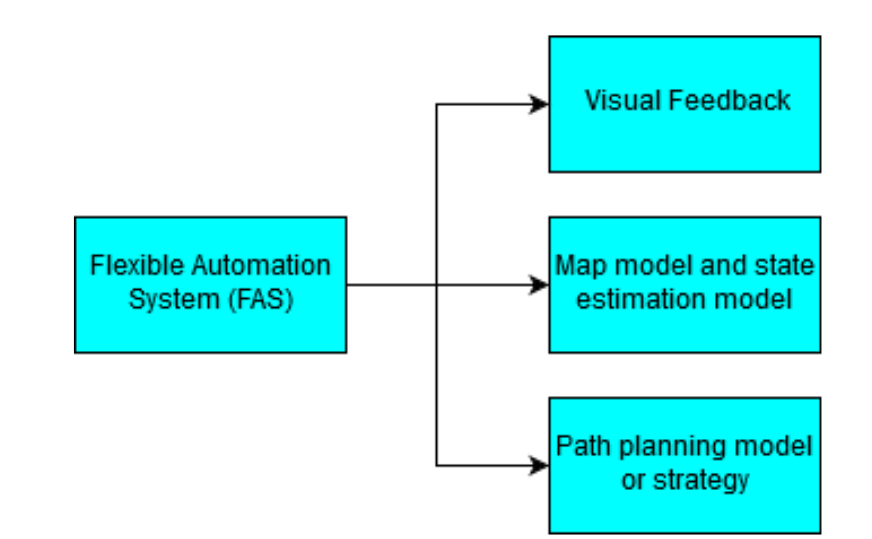
\includegraphics[width=\linewidth]{\thesisDir/chapter1/figures/fas.png}
  \caption{Three aspects of an FAS to maintain a safe and cost effective robotic system in a production
line.}
  \label{fig:fas}
\end{figure}

The FAS uses visual feedback, such as visual camera, laser range finder, or a visual-depth
camera, to model the workspace and to model the state of the robot.

The second aspect of an FAS is the state estimation model and the map model summarized by figure
\ref{fig:map_state_blocks}. A map model is a mathematical representation of an environment and state estimation model is
a process of estimating an industrial robot configuration, location, velocity and acceleration of its end
effector. The map model will provide the information for the FAS to manage the movement of a robot
arm in its workspace based on the state estimation.
\begin{figure}
  \centering
  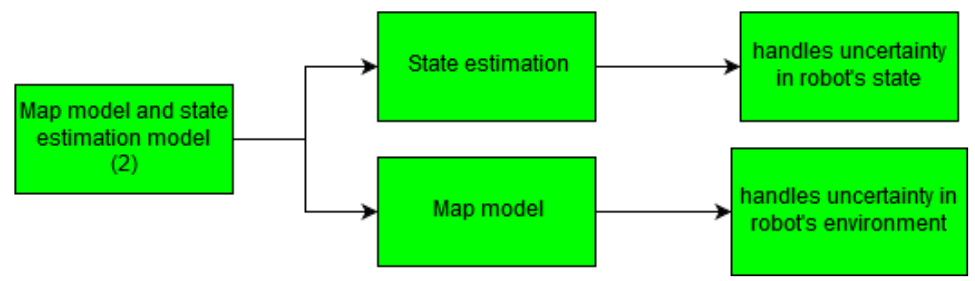
\includegraphics[width=\linewidth]{\thesisDir/chapter1/figures/map_state_blocks.png}
  \caption{The second aspect of an FAS consist of two mathematical model that manage the uncertainty
of the workspace of a robot and the uncertainty of the state of the robot.}
  \label{fig:map_state_blocks}
\end{figure}

The third aspect of an FAS is the path-planning model. 
The path-planning model is used to calculate a
way to reach a point in space without colliding with any obstructions or obstacles. The path is dependent
on the information restored in the map model of the workspace.

\section{The Motivation of Eye-in-Hand Robot Configuration}\label{sec:motive_eyehand}
Placement of the machine vision and the decision of the 
placement of the vision is non-trivial.
The designer can consider, eye-to-hand configuration where the vision sensor is attached to an additional
structure that has a vantage point of the robot manipulator and the workspace \parencite{Luo2016} or an
eye-in-hand configuration where a vision sensor is place on
the robot's end-effector or at the last link of the robot arm.
The latter configuration requires
no additional structure 
and the visual feedback can be used as a state estimator 
and a mapping tool abiding the movement of the robot. This 
makes eye-in-hand configuration more space-efficient. Unlike
eye-to-hand configuration, eye-in-hand sensors provide more
information gain in terms of the state of the robot and the
environment. The feedback from eye-in-hand configuration
lacks visual-obstruction where more than 
one vantage point can be achieve when the sensors move 
with the end effector. The sensor in eye-in-hand configuration
aids task involving reaching and manipulating since both tasks
are specific to the end-effector. In the case of eye-to-hand 
configuration, both reaching and manipulation may be subjected
to visual obstruction and extra rigs for the sensor. 

As an example, \textcite{Luo2016}
used Microsoft's Kinect, 
a type of visual-depth sensor \acrfull{RGB-D}, 
to produce workspace
model of their robot system and to identify objects 
in the workspace. Figure \ref{fig:eye2hand} shows the rigidity
of their setup.

\textcite{Klingensmith2016} uses the eye-in-hand configuration
where an RGB-D sensor is connected at the end effector to
auto-calibrate the robot's position and configuration
illustrated in figure \ref{fig:eyeINhand}. Extra structures
were observed in the figure but in this stage of their research, 
their eye-to-hand sensor setup are not reported in their findings. 

\begin{figure}
  \centering
  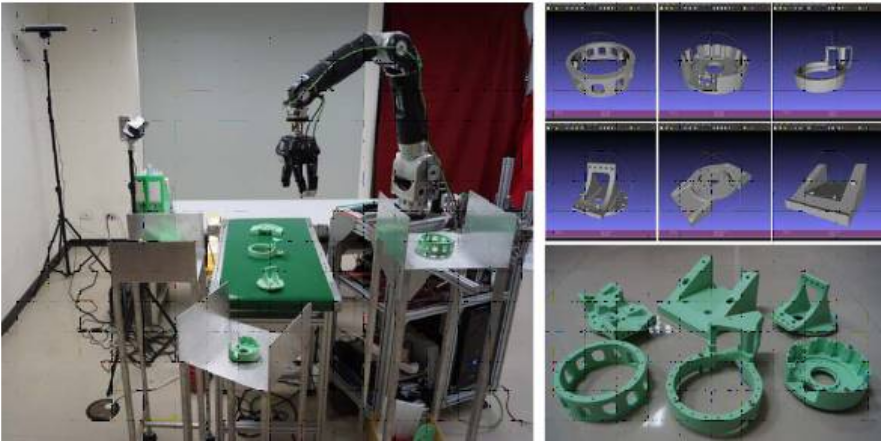
\includegraphics[width=\linewidth]{\thesisDir/chapter1/figures/eye2hand.png}
  \caption{Eye-in-hand configuration that uses visual feedback enables an articulated robotic
arm to identify objects in its workspace for manipulation.}
  \label{fig:eye2hand}
\end{figure}

\import{\thesisDir/chapter1/figures/}{eyeINhand.tex}
\section{The Devoid of Unified Solution for 
Uncertainty Management in State and Workspace of an Industrial Robot}
\label{sec:ununified_sol}
\import{\thesisDir/chapter1/figures/}{fas_slam.tex}

Despite rich solution options to uncertainty of a robot state and its environment, the solutions are disjoint
and performed separately. SLAM, however,
incorporate both the solution to uncertainty of the robot's state and the solution to uncertainty of the
environment into one framework. Equation \ref{eq:slam_eq} summarize the concept of SLAM:

\begin{equation}
  \label{eq:slam_eq}
  p(m_i,x_i|z_i,u_i,x_{i-1})
\end{equation}

where $\gls{p}$ (also known as posterior) is the process of maintaining the map of an unknown
environment and estimating the current 
state or pose of a robot. 
$\gls{mi} \in \mathbb{R}^{3n}$, is the global map model, $x_i \in \mathbb{R}^3 \times \vb*{SO(3)}$
is the state estimation, $\gls{zi}$ is the measurement or observation model or visual feedback model of the robot, and 
$ \gls{ui} $ is the state transition matrix or state transition model of the robot. $x_{i-1}$ before a new
measurement is taken. Figure \ref{fig:slam_posterior} summarizes the arguments of equation \ref{eq:slam_eq}.

\begin{figure}
  \centering
  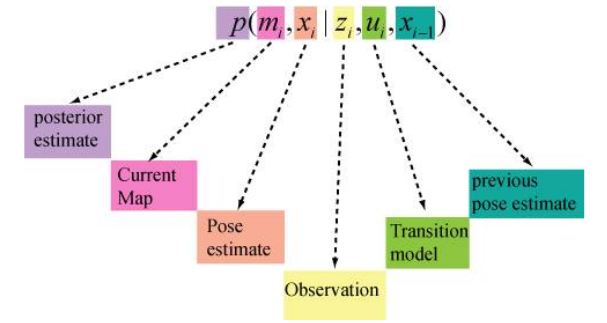
\includegraphics[width=\linewidth]{\thesisDir/chapter1/figures/slam_posterior.png}
  \caption{The variables parameterizing the SLAM solution }
  \label{fig:slam_posterior}
\end{figure}

\import{\thesisDir/chapter1/figures/}{research_gap.tex}


In theory a SLAM solution covers the first and the second aspects of the FAS proposed in this research.
Figure \ref{fig:fas_slam} articulates the relevance of SLAM solution to an FAS.

Yet SLAM has only been optimized specifically for autonomous robot to address an unknown
environment. The definitive researches on the use of SLAM in articulated robot were introduced by 
\textcite{Klingensmith2016}, \textcite{Li2019c}, and \textcite{Ito2020}. However, they
did not consider the uncertainty of the state of the robot, the uncertainty of 
the robot’s environment, and
the path planning solution in a single framework. Figure \ref{fig:research_gap} 
summarizes the gap in finding a solution to a path-planning under the uncertainty of
the state of the robot and the uncertainty of its environment.


\section{Problem Statement and its Significance}\label{sec:problem_statement}
The current state-of-the-art approaches to an industrial articulated manipulator lack a 
solution that addresses the the safety of the system in a changing environment. 
SLAM solutions for articulated manipulator have only addressed 
the issues of accuracy without tackling the high maintenance cost and safety of a robot manipulator specifically 
on the production set-up. 
Furthemore, the performance of these solutions against  probabilistic path-planner for robot manipulator has
yet been reported. 
This research intend to aspire flexibility and cost effective
robot manipulator system for industrial purposes in SME's using
sampling-based planner closely coupled with a SLAM solution.

\section{Research Philosphy}\label{sec:research_philosophy}
A compliant robotic arm by leveraging the probabilistic mathematical models for map
of an environment, the state estimation of a robot, and the path-planning model in controlling the robot motion
sustains safety operation and cost-effective production line for
SME's.

\section{Objectives}\label{sec:objectives}
\begin{enumerate}
  \item \label{objective1} 
    To design a six-axis manipulator and build it as a prototype
    of a compliant manipulator.
   \item \label{objective2} To simulate a moving obstacle avoidance capability using a probabilistic planner.
  \item \label{objective3} To demonstrate the obstacle avoidance capability on
    the compliant manipulator hardware with a synthetic moving obstacle augmented from a simulated environment.
  \item \label{objective4} To show the feasibility of using a SLAM solution 
    as a feedback pipeline in motion planning.

\end{enumerate}

\section{Research Scope}
This research uses a back-drivable (compliant) articulated robot with six axes to implement the framework of a
fully probabilistic strategy to path-planning and obstacle avoidance. This research only use an RGB-D sensor.

The dynamic environment is a non-reflective and non-specular workspace. 
In context of designing the workspace as a dynamic environment, 
the workspace is not share
with another robotic arm. Instead, the workspace will be introduced with a moving obstacle. 
Figure \ref{fig:research_scope}
shows the scope and the considerations of this research.

\begin{figure}[h]
  \centering
  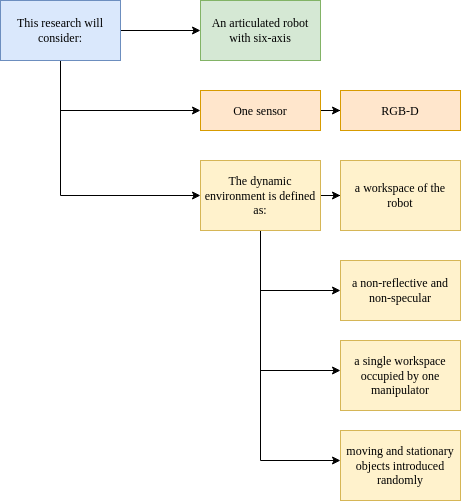
\includegraphics[width=\linewidth]{\thesisDir/chapter1/figures/research_scope2.png}
  \caption{The scope of this research and its considerations}
  \label{fig:research_scope}
\end{figure}

\section{Methodology}\label{sec:methodology}

In this research, the model of a robot kinematics, specifically
on the task space (the end-effector frame) of the robot, 
${C}_{ee} \in \mathbb{R}^3 \cross \gls{SO3}$ where, 
$\mathbb{R}^3 \cross \vb*{SO(3)}$ is homeomorphic to the special 
Euclidean group, $\gls{SE3}$. 
Hence, given $\{{C}_{ee}=c_{ee}\}$, the task space 
of the robot manipulator is a set in equation \ref{eq:se3}:

\import{\thesisDir/chapter1/equations/}{se3.tex}
%this needs revision
%\begin{equation}
%  \label{eq:se3}
%  \{c_{ee} = (t,R): t \in \mathbb{R}^3, R \in \vb*{SO(3)}\}
%\end{equation}
where $\gls{rotationMatrix}$ is the rotation matrix and
\gls{translationVector} is the translation in 3D.
Thus, since all SLAM solutions for three-dimensional space provide state estimation in the form of 
$ \gls{R3} \cross \gls{SO3}$, their model in equation 
\ref{eq:slam_eq} holds
for industrial robot arm. 
Nonetheless, the complete solution for SLAM does not consider 
the path-planning model of the robot arm, specifically, 
the mapping of control space,
${C}^n \in \mathbb{R}^n$ into the $\gls{Configurationee}$, where 
$n$ is the number of rigid body in the robotic arm. 
Hence, I will investigate the tractability of reconciling
probabilistic model of a path-planning strategy
with Equation \ref{eq:slam_eq} such that:

\begin{equation} \label{eq:splam_eq}
  p(\mu_i,m | \hat{x_i},z_i,u_i)
\end{equation}

where $p$ is similar to the process of maintaining the map 
of a the workspace and estimating the
state of a robot concurrently where, $\gls{xestimate}$, 
is the state estimation 
pipeline of a SLAM solution in equation \ref{eq:slam_eq}.

In equation \ref{eq:splam_eq}, the solution incorporates both 
SLAM algorithm and a probabilistic path-planning
model into a single framework instead of considering the SLAM 
solution and path-planning algorithm separately. 
I outline my research methodology based on equation \ref{eq:splam_eq}. An overview of the research methodology against 
the objectives of this research is presented in figure \ref{fig:methodology_objective}.

%These subsections are not needed
%in this chapter so I will 
% put it under \iffalse environment
% if needed, active them 
% by replacing \iffalse with \iftrue

\iffalse

\subsection{Feedback Modeling ($z_i$)}\label{feedback_modeling_methodology}
The feedback model uses only one sensor; the RGB-D sensor. This
research will model the RGB-D sensor based on their statistical parameter 
estimation method
prescribed in \textcite{Iman2016}.
The data from the RGB-D sensors will represent the sensor model, $z_i$ .

\subsection{Map Modeling ($m_i$)}\label{map_modeling_methodology}
The obstacle presented to the workspace will be modeled and tracked based on the probabilistic model of
the map of the environment using the octomap map model. 

\subsection{State Estimation Modeling ($x_i$)}\label{state_estimation_methodology}
The state estimation model is based on features extraction from the map model where each joints of the
articulated robot arm is estimated from the visual feedback model and compared with its the planner's solution.

\subsection{Articulated Robot Transition Matrix Modeling ($u_i$)}\label{transition_matrix_methodology}
The robot forward and inverse kinematics model of the robot will be used as the process model or the
transition matrix of the system. A process model or a transition model is a deterministic representation of
the robot’s motion and configurations. I
will adopt the total algebraic solution to the inverse kinemtatic delineated by \textcite{Pires2007}

\subsection{SLAM Solution and Path Planning Model ($\gls{mui}$)}\label{path_planning_methodology}
Both the solution of the planner and the state estimation of the SLAM pipeline will be compared and analysis to see if it is feasible 
for both algorithms to be combined as a unified solution represented by the
model in equation \ref{splam_eq}

\subsection{ROS Middleware Implementation}\label{implementation_methodology}
The mathematical models: $z_i$ , $m_i$ , $x_i$ , $u_i$ , $\mu_i$ , will be programmatically translated into a Robotic Operating
System (ROS) package. The ROS middleware is essential in integrating the articulated robot chassis
with the mathematical model of the map, visual feedback sensor, state estimation, transition matrix and
the probabilistic path-planning.

\subsection{Validation and Evaluation}\label{sec:validation_methodology}
The ROS package containing the availabe path-planning strategy will then be used in a simulation
using the Gazebo software available in the ROS middleware. The parameters from this simulation will be
used in an experimental setup that introduces various obstacles to the workspace of the articulated robot
arm. This series of experiments will determine the efficiency of various filtering and modeling techniques
for the path-planning strategy.

\fi

\section{The Outline of the Thesis}\label{sec:thesis_outline}
In this chapter, the concept of FAS is translated into
formulating a SLAM solution for a robot manipulator. 
This thesis will elucidate  the SLAM-planner 
coupling and pipelininig in the coming chapters.
The reader is usher to a literature review 
of the state-of-the-art and the 
leading papers on state estimation, map-building models and path-planning in \autoref{chap:lit_review}.
The readers are then introduced with 
the mathematical foundation
in \autoref{chap:mathematical_background}.
In \autoref{chap:experimentation_result_discussion}, the experimentation are delineated and the chapter continues with 
the discussion on the findings and result. 
This thesis concludes with 
\autoref{chap:conclusion_recommendation} with recommendation 
on future works. 

\begin{figure}[h]
  \centering
  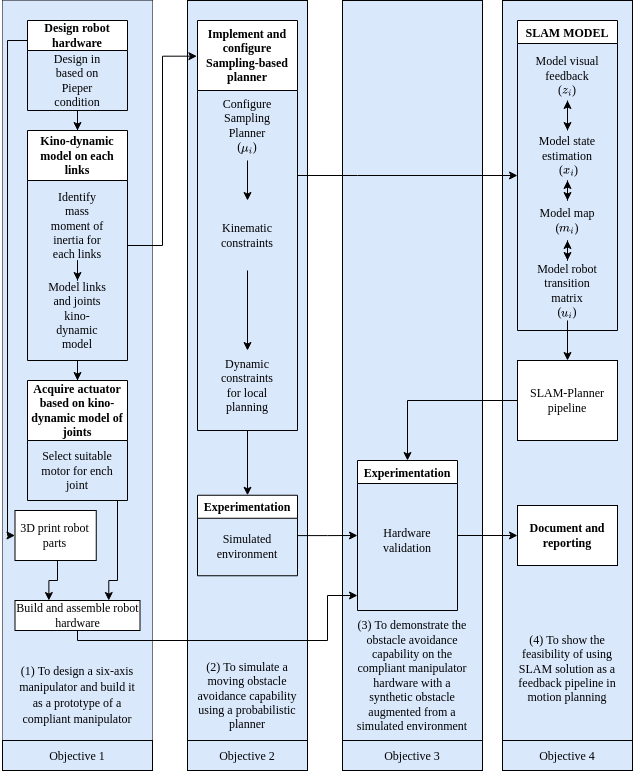
\includegraphics[width=\linewidth]{\thesisDir/chapter1/figures/methodology_objective2.png}
  \caption{Summary of the methodology to achieve the objectives of this research}
  \label{fig:methodology_objective}
\end{figure}



\ifwhole\else
	\printbibliography
	\end{document}
\fi


